{
Giver man tre forskellige mennesker den opgave at afgøre hvad der er det
interessante i et givet maleri, kan man meget vel få tre forskellige
svar. Mere kompliceret bliver det når man spørger ind til \emph{hvordan}
de er kommet frem til deres svar. Én begrunder måske sit valg med en
viden om netop det givne maleri, en anden med viden om maleriets
kunstner eller periode, mens en tredie begrunder det med æstetiske
virkemidler eller subjektive holdninger. Her er alle muligheder åbne for
at lave fejl, da man som regel ikke har kunstneren til rådighed til at
give det rigtige svar, hvis han da overhovedet selv kender det.
Maleriets motiv kan lede én på sporet af hvad der er interessant, men
dette kræver måske en viden om motivets bagvedliggende historie.
Mennesket tager altså en lang række overvejelser og baggrundsviden i
betragtning når ovenstående opgave skal løses.

Det interessante i et billede afhænger af den enkelte opgave.  Hvis vi
forestiller os en læge der kigger på et røntgenbillede af en patient som
har brækket armen, er det indlysende hvad lægen betragter som det
interessante i billedet, nemlig der hvor bruddet sidder. Når vi har med
tilfældige malerier at gøre, så står vi dog stadig tilbage med
spørgsmålet: \emph{``Hvad er egentlig \emph{interessant} i et maleri?''}
Vi lader dette spørgsmål stå åbent for at se på hvordan computeren
betragter et maleri.

\begin{figure}[h]
    \centering
    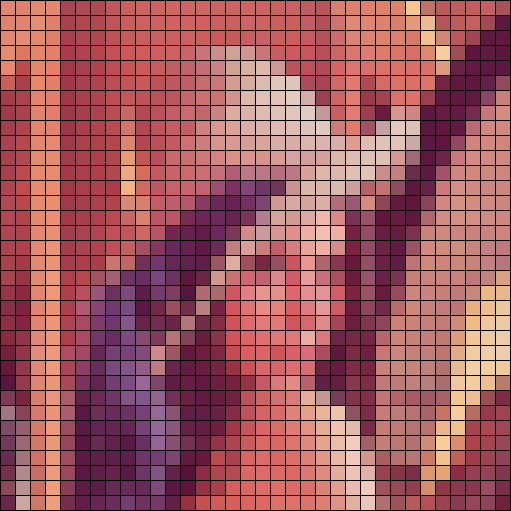
\includegraphics[scale=0.3]{afsnit/baggrund/billeder/pixel_lena}
    \caption[]{Pixels i et billede}
    \label{pixel_lena}
\end{figure}

Billedet i figur \ref{pixel_lena} er blevet delt op i nogle små felter
kaldet pixels. Hver pixel har en farve. Computeren opfatter et billede
netop som pixels. Computeren ser endvidere disse pixels \emph{én ad
gangen}. Det svarer altså til at den enkelte farve til en pixel bliver
læst op for en person der ikke kan se selve billedet. For at køre
eksemplet helt ud, så har vi at en person får følgende at vide:
\begin{quote}
    \emph{``Pixel med koordinater $(0, 0)$ er gul. Pixel med
    koordinater $(1, 0)$ er orange''} etc.
\end{quote}
Dette giver ingen egentlig information om \emph{hvad} billedet
forestiller. Computeren kan ikke se billedet i sin helhed og har som
udgangspunkt ikke nogen baggrundsviden at basere en vurdering på. Det
eneste computeren kan gøre er at gå billedet igennem pixel for pixel og
sammenligne dem.

Vi ønsker at bruge computeren til at afgøre om der ligger noget
interessant i billedet omkring det gyldne snit. Vi vil derfor nu kaste
et blik på den forskning der allerede er blevet gjort på dette område.

}

% vim: set tw=72 spell spelllang=da:
